\section{Link Layer Architecture}

The link layer implements the single-hop communication behavior needed by the upper stack, while keeping a
strict boundary from routing and application logic. Its main job is to provide dependable one-hop delivery on a
constrained long-range channel. This includes frame construction, channel access coordination, reception
handling, and energy-aware behavior. In our design, upper layers submit payloads and receive delivery events
through an asynchronous service interface, while all radio-facing behavior stays inside the link layer. This
separation lets forwarding policy and application logic evolve without being tightly coupled to modem-specific
constraints.

The wire format uses a compact fixed-size header followed by a bounded payload region. This keeps parsing
deterministic and makes interoperability across nodes explicit. The header encodes source and destination
identifiers, message classification, sequence numbering, control flags, and payload length. For addressing, we
use node-local unicast identifiers and a dedicated broadcast destination value for one-to-many dissemination.
Sequence and flag metadata support reliability signaling when needed, without adding mandatory overhead for
every traffic class. We also reserve a message type for acknowledgment control traffic, so ACK signaling is not
confused with application-defined data categories.

Medium access control uses a listen-before-send strategy based on channel activity detection. Before sending,
the transmitter checks for channel occupancy and defers when LoRa activity is detected, which reduces
collision probability on a shared medium. If the channel is repeatedly busy, we apply bounded retry behavior
with randomized backoff to reduce synchronization between concurrent transmitters. If the medium stays
unavailable beyond the configured sensing budget, the pending transmission is discarded so latency does not
grow without bound and the queues do not become unstable. Overall, we prefer predictable timing and spectrum
discipline over aggressive persistence. The runtime state transitions are shown in
Fig.~\ref{fig:link-layer-state-machine}.

\begin{figure*}[!t]
\centering
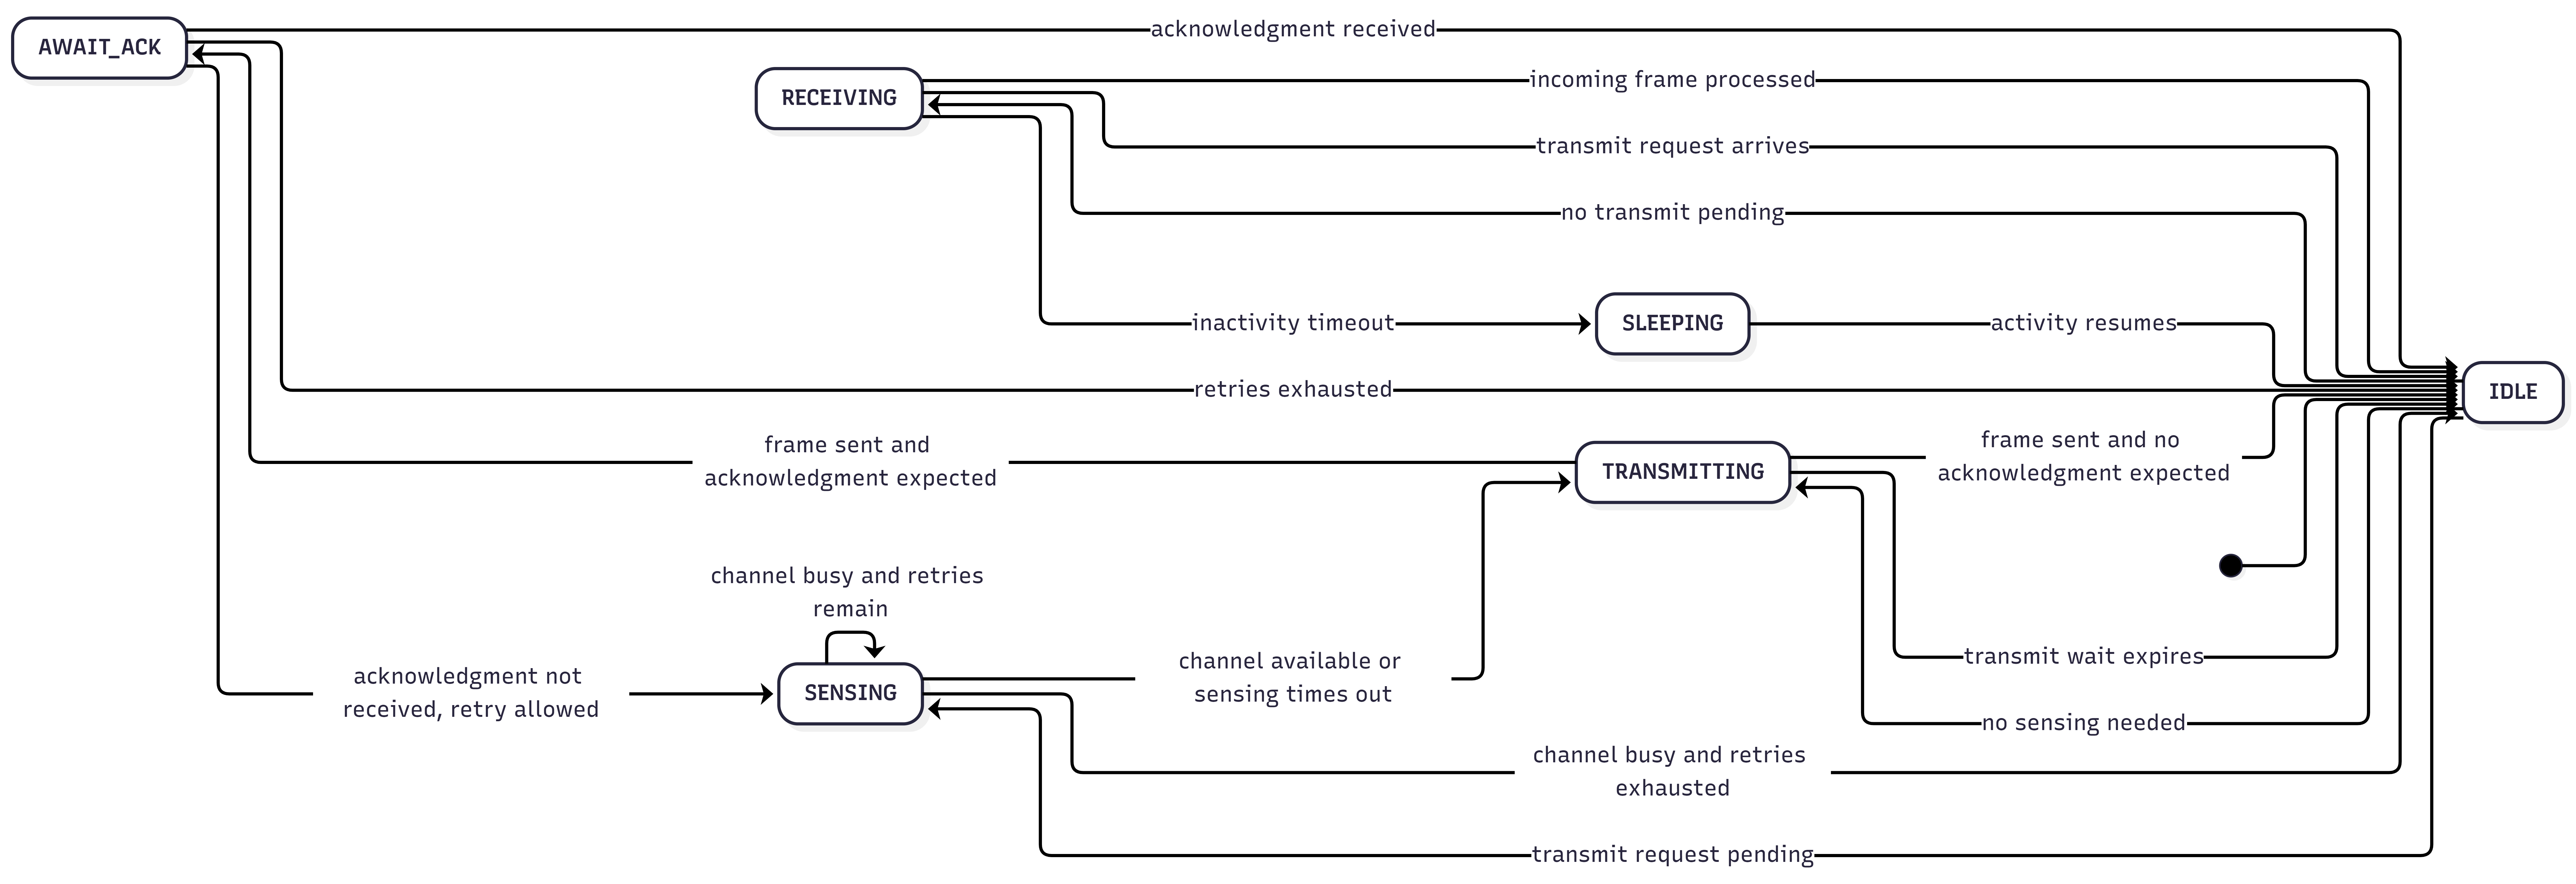
\includegraphics[width=0.95\textwidth]{assets/architecture/link_layer_state_machine.png}
\caption{Link-layer runtime state machine showing transitions among reception, channel activity detection,
transmission wait, acknowledgment wait, sleep control, and idle handling.}
\label{fig:link-layer-state-machine}
\end{figure*}

The transmission workflow combines queued frame dispatch with optional per-frame reliability. Once a frame is
admitted for transmission, it goes through channel sensing and, if the channel is clear, it is transmitted over
the radio interface. For traffic that does not request reliability, we finish once the transmit confirmation is
received. For reliability-enabled traffic, the sender enters a bounded acknowledgment wait phase and checks
incoming acknowledgments against the sequence and addressing context. A valid match ends the transaction and a
positive outcome is reported to the upper layer. If there is a timeout, we do controlled retransmissions up to
the configured maximum, after which the frame is reported as undelivered. This selective reliability model lets
critical safety messages request stronger delivery assurance while keeping lower overhead for noncritical
traffic, as shown in Fig.~\ref{fig:link-layer-sequence}.

\begin{figure*}[!t]
\centering
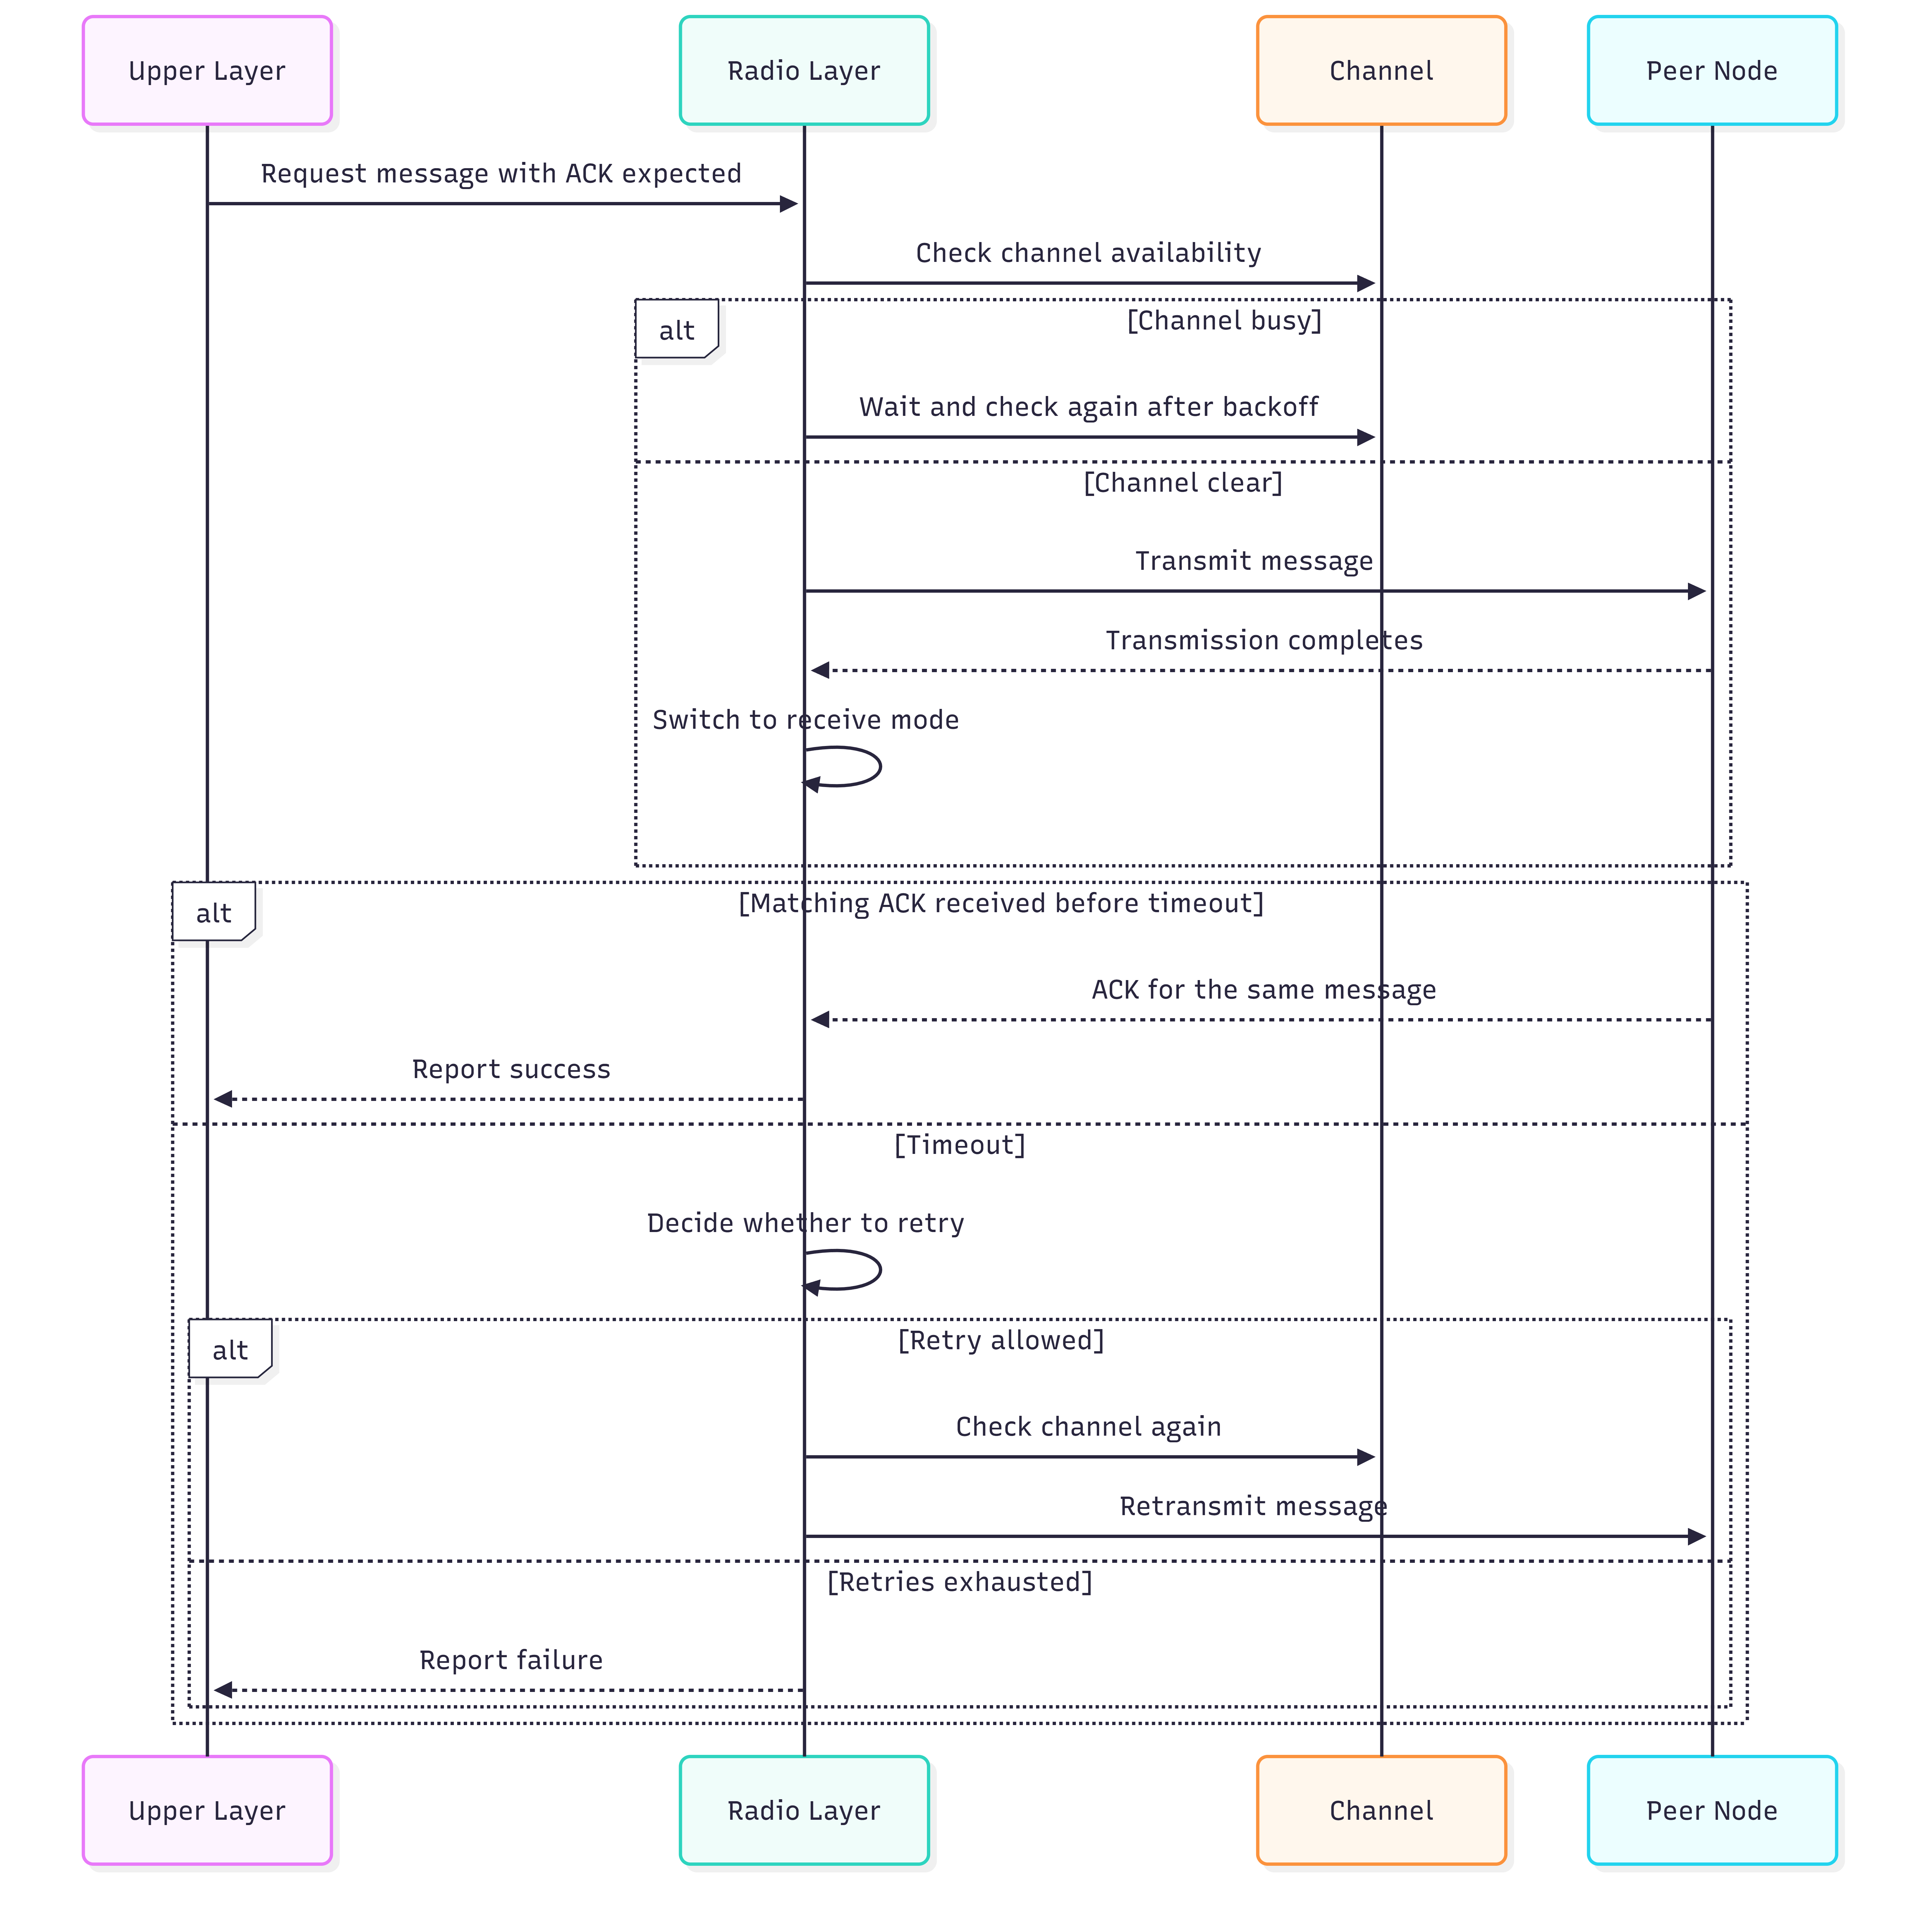
\includegraphics[width=0.7\textwidth]{assets/architecture/link_layer_seq.png}
\caption{Acknowledgment-enabled transmit sequence at the link layer, including CAD-based channel access,
transmission completion handling, ACK validation, timeout detection, and bounded retransmission.}
\label{fig:link-layer-sequence}
\end{figure*}

Inbound processing follows a strict filtering pipeline so upper layers do not have to deal with malformed or
irrelevant traffic. Frames below the minimum valid length are rejected immediately. Valid frames are parsed
and link-quality observations are recorded for neighbor awareness. Destination filtering then removes packets
that are not addressed to the local node or the broadcast group. Pure acknowledgment frames are handled
internally by the reliability subsystem and are not exposed as application payload events. If a received data
frame requested acknowledgment, we generate the corresponding acknowledgment response at link level. Only
after these checks pass do we deliver payload data upward, so upper layers only see semantically meaningful
and policy-compliant traffic.

Energy management is handled through adaptive receive-idle control. The receiver stays active to remain
responsive, but it transitions to a low-power modem state after sustained inactivity. Wake-up is event-driven:
outbound traffic demand or relevant radio interrupt activity restores active operation and normal processing.
This balances readiness and battery efficiency for vehicular platforms that may need to operate for long
intervals without missing important events.

Hardware abstraction is done through a backend interface that separates protocol/state logic from the
transceiver drivers. The link layer uses this interface for channel sensing, transmission, reception,
signal-quality observation, interrupt signaling, and power-state transitions. Because of this, the same
link-layer behavior can run against real radio hardware or controlled test backends without changing the
architecture. This improves portability, supports deterministic validation in the lab, and reduces coupling
between communication policy and platform-specific implementation details.

